\documentclass[]{extarticle}
\usepackage{lmodern}
\usepackage{amssymb,amsmath}
\usepackage{ifxetex,ifluatex}
\usepackage{fixltx2e} % provides \textsubscript
\ifnum 0\ifxetex 1\fi\ifluatex 1\fi=0 % if pdftex
  \usepackage[T1]{fontenc}
  \usepackage[utf8]{inputenc}
\else % if luatex or xelatex
  \ifxetex
    \usepackage{mathspec}
  \else
    \usepackage{fontspec}
  \fi
  \defaultfontfeatures{Ligatures=TeX,Scale=MatchLowercase}
\fi
% use upquote if available, for straight quotes in verbatim environments
\IfFileExists{upquote.sty}{\usepackage{upquote}}{}
% use microtype if available
\IfFileExists{microtype.sty}{%
\usepackage{microtype}
\UseMicrotypeSet[protrusion]{basicmath} % disable protrusion for tt fonts
}{}
\usepackage[margin=0.6in]{geometry}
\usepackage{hyperref}
\hypersetup{unicode=true,
            pdftitle={Chapter 11: Outliers and Influential Observations},
            pdfborder={0 0 0},
            breaklinks=true}
\urlstyle{same}  % don't use monospace font for urls
\usepackage{color}
\usepackage{fancyvrb}
\newcommand{\VerbBar}{|}
\newcommand{\VERB}{\Verb[commandchars=\\\{\}]}
\DefineVerbatimEnvironment{Highlighting}{Verbatim}{commandchars=\\\{\}}
% Add ',fontsize=\small' for more characters per line
\usepackage{framed}
\definecolor{shadecolor}{RGB}{248,248,248}
\newenvironment{Shaded}{\begin{snugshade}}{\end{snugshade}}
\newcommand{\KeywordTok}[1]{\textcolor[rgb]{0.13,0.29,0.53}{\textbf{#1}}}
\newcommand{\DataTypeTok}[1]{\textcolor[rgb]{0.13,0.29,0.53}{#1}}
\newcommand{\DecValTok}[1]{\textcolor[rgb]{0.00,0.00,0.81}{#1}}
\newcommand{\BaseNTok}[1]{\textcolor[rgb]{0.00,0.00,0.81}{#1}}
\newcommand{\FloatTok}[1]{\textcolor[rgb]{0.00,0.00,0.81}{#1}}
\newcommand{\ConstantTok}[1]{\textcolor[rgb]{0.00,0.00,0.00}{#1}}
\newcommand{\CharTok}[1]{\textcolor[rgb]{0.31,0.60,0.02}{#1}}
\newcommand{\SpecialCharTok}[1]{\textcolor[rgb]{0.00,0.00,0.00}{#1}}
\newcommand{\StringTok}[1]{\textcolor[rgb]{0.31,0.60,0.02}{#1}}
\newcommand{\VerbatimStringTok}[1]{\textcolor[rgb]{0.31,0.60,0.02}{#1}}
\newcommand{\SpecialStringTok}[1]{\textcolor[rgb]{0.31,0.60,0.02}{#1}}
\newcommand{\ImportTok}[1]{#1}
\newcommand{\CommentTok}[1]{\textcolor[rgb]{0.56,0.35,0.01}{\textit{#1}}}
\newcommand{\DocumentationTok}[1]{\textcolor[rgb]{0.56,0.35,0.01}{\textbf{\textit{#1}}}}
\newcommand{\AnnotationTok}[1]{\textcolor[rgb]{0.56,0.35,0.01}{\textbf{\textit{#1}}}}
\newcommand{\CommentVarTok}[1]{\textcolor[rgb]{0.56,0.35,0.01}{\textbf{\textit{#1}}}}
\newcommand{\OtherTok}[1]{\textcolor[rgb]{0.56,0.35,0.01}{#1}}
\newcommand{\FunctionTok}[1]{\textcolor[rgb]{0.00,0.00,0.00}{#1}}
\newcommand{\VariableTok}[1]{\textcolor[rgb]{0.00,0.00,0.00}{#1}}
\newcommand{\ControlFlowTok}[1]{\textcolor[rgb]{0.13,0.29,0.53}{\textbf{#1}}}
\newcommand{\OperatorTok}[1]{\textcolor[rgb]{0.81,0.36,0.00}{\textbf{#1}}}
\newcommand{\BuiltInTok}[1]{#1}
\newcommand{\ExtensionTok}[1]{#1}
\newcommand{\PreprocessorTok}[1]{\textcolor[rgb]{0.56,0.35,0.01}{\textit{#1}}}
\newcommand{\AttributeTok}[1]{\textcolor[rgb]{0.77,0.63,0.00}{#1}}
\newcommand{\RegionMarkerTok}[1]{#1}
\newcommand{\InformationTok}[1]{\textcolor[rgb]{0.56,0.35,0.01}{\textbf{\textit{#1}}}}
\newcommand{\WarningTok}[1]{\textcolor[rgb]{0.56,0.35,0.01}{\textbf{\textit{#1}}}}
\newcommand{\AlertTok}[1]{\textcolor[rgb]{0.94,0.16,0.16}{#1}}
\newcommand{\ErrorTok}[1]{\textcolor[rgb]{0.64,0.00,0.00}{\textbf{#1}}}
\newcommand{\NormalTok}[1]{#1}
\usepackage{graphicx,grffile}
\makeatletter
\def\maxwidth{\ifdim\Gin@nat@width>\linewidth\linewidth\else\Gin@nat@width\fi}
\def\maxheight{\ifdim\Gin@nat@height>\textheight\textheight\else\Gin@nat@height\fi}
\makeatother
% Scale images if necessary, so that they will not overflow the page
% margins by default, and it is still possible to overwrite the defaults
% using explicit options in \includegraphics[width, height, ...]{}
\setkeys{Gin}{width=\maxwidth,height=\maxheight,keepaspectratio}
\IfFileExists{parskip.sty}{%
\usepackage{parskip}
}{% else
\setlength{\parindent}{0pt}
\setlength{\parskip}{6pt plus 2pt minus 1pt}
}
\setlength{\emergencystretch}{3em}  % prevent overfull lines
\providecommand{\tightlist}{%
  \setlength{\itemsep}{0pt}\setlength{\parskip}{0pt}}
\setcounter{secnumdepth}{0}
% Redefines (sub)paragraphs to behave more like sections
\ifx\paragraph\undefined\else
\let\oldparagraph\paragraph
\renewcommand{\paragraph}[1]{\oldparagraph{#1}\mbox{}}
\fi
\ifx\subparagraph\undefined\else
\let\oldsubparagraph\subparagraph
\renewcommand{\subparagraph}[1]{\oldsubparagraph{#1}\mbox{}}
\fi

%%% Use protect on footnotes to avoid problems with footnotes in titles
\let\rmarkdownfootnote\footnote%
\def\footnote{\protect\rmarkdownfootnote}

%%% Change title format to be more compact
\usepackage{titling}

% Create subtitle command for use in maketitle
\newcommand{\subtitle}[1]{
  \posttitle{
    \begin{center}\large#1\end{center}
    }
}

\setlength{\droptitle}{-2em}

  \title{Chapter 11: Outliers and Influential Observations}
    \pretitle{\vspace{\droptitle}\centering\huge}
  \posttitle{\par}
    \author{}
    \preauthor{}\postauthor{}
    \date{}
    \predate{}\postdate{}
  
\usepackage{soul}
\usepackage{booktabs}

\begin{document}
\maketitle

\subsubsection{Recall Anscombe's Data}\label{recall-anscombes-data}

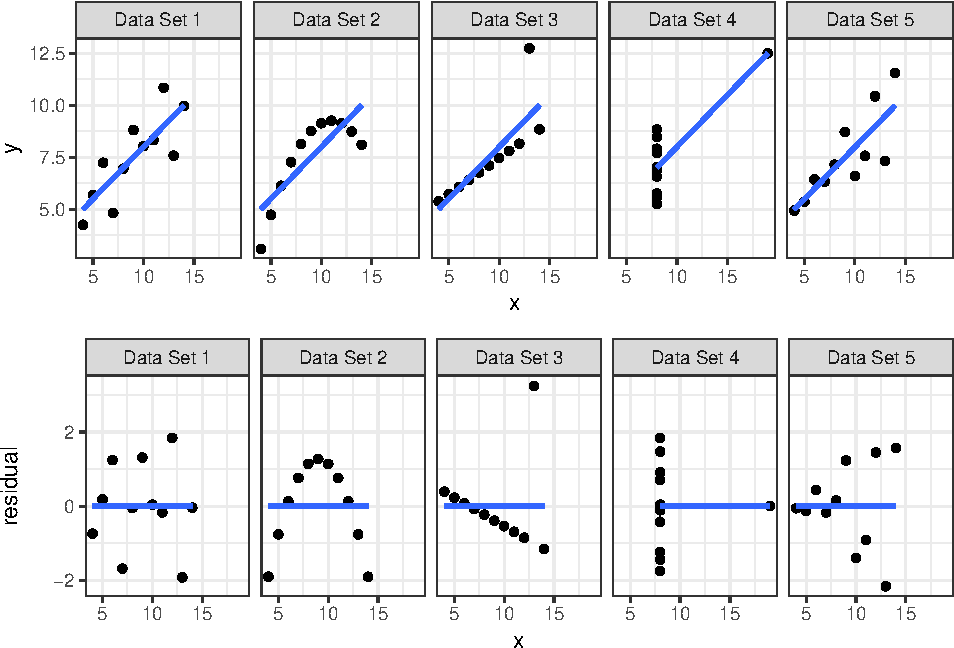
\includegraphics{20190417_residual_diagnostics_files/figure-latex/unnamed-chunk-1-1.pdf}

\begin{itemize}
\tightlist
\item
  For today, let's focus on Data Sets 3 and 4
\item
  Definitions (note: there are not universally agreed on definitions for
  these terms):

  \begin{itemize}
  \tightlist
  \item
    An \textbf{outlier} is an observation that ``doesn't fit'' with the
    patterns in the rest of the data

    \begin{itemize}
    \tightlist
    \item
      Both data set 3 and data set 4 have outliers
    \end{itemize}
  \item
    An \textbf{influential observation} is an observation whose removal
    from the data set would substantially change the model fit
    (coefficient estimates)

    \begin{itemize}
    \tightlist
    \item
      Both data set 3 and data set 4 have influential observations
    \item
      The point in data set 4 is \emph{more influential}
    \end{itemize}
  \item
    A \textbf{high leverage observation} is one whose explanatory
    variable values are far from the explanatory variable values of
    other observations

    \begin{itemize}
    \tightlist
    \item
      Data set 4 has a high leverage observation
    \item
      Data set 3 does not
    \end{itemize}
  \end{itemize}
\item
  Note that residual plots \textbf{exactly fail} to identify very
  influential/high leverage observations!!!
\end{itemize}

\newpage

\subsection{Leverage}\label{leverage}

\begin{itemize}
\tightlist
\item
  If the model has 1 \(X\) variable, the leverage of observation \(i\)
  is defined to be
\end{itemize}

\(h_i = \frac{(X_i - \bar{X})^2}{\sum_{j=1}^n (X_j - \bar{X})^2} + \frac{1}{n}\)

\begin{itemize}
\tightlist
\item
  Basically, how far is \(X_i\) from \(\bar{X}\), standardized in an
  obsure way.

  \begin{itemize}
  \tightlist
  \item
    \(\frac{1}{n} \leq h_i \leq 1\)
  \item
    Average of leverages is \(p/n\) (where \(p\) is the number of
    parameters for the mean in the model).
  \end{itemize}
\item
  As a very rough guide, \(h_i > 2p/n\) indicates an observation is
  worth looking into more
\end{itemize}

Plots of leverage vs.~observation index (code will be shown later)

\begin{Shaded}
\begin{Highlighting}[]
\CommentTok{# 2p/n; p = 2 since we have beta_0 and beta_1 in our simple linear regression model}
\DecValTok{2} \OperatorTok{*}\StringTok{ }\DecValTok{2} \OperatorTok{/}\StringTok{ }\KeywordTok{nrow}\NormalTok{(anscombe)}
\end{Highlighting}
\end{Shaded}

\begin{verbatim}
## [1] 0.3636364
\end{verbatim}

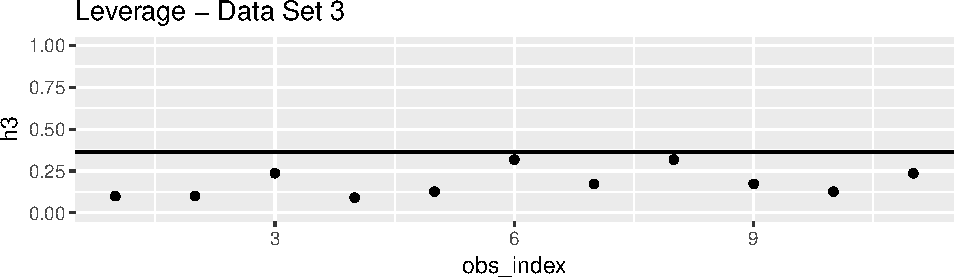
\includegraphics{20190417_residual_diagnostics_files/figure-latex/unnamed-chunk-3-1.pdf}

Looks OK

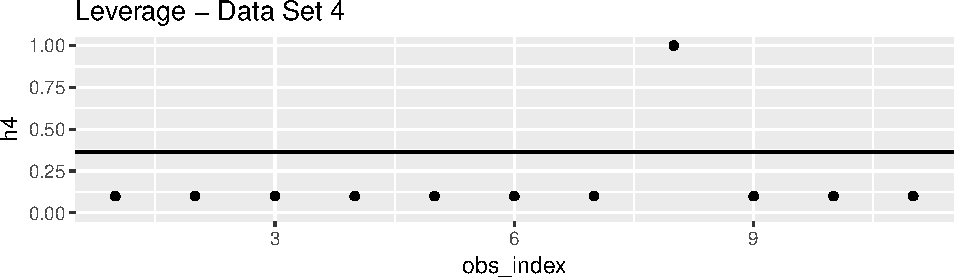
\includegraphics{20190417_residual_diagnostics_files/figure-latex/unnamed-chunk-4-1.pdf}

\begin{Shaded}
\begin{Highlighting}[]
\CommentTok{# confirm observation 8 is the one with a big X!}
\NormalTok{anscombe}\OperatorTok{$}\NormalTok{x4[}\DecValTok{8}\NormalTok{]}
\end{Highlighting}
\end{Shaded}

\begin{verbatim}
## [1] 19
\end{verbatim}

\newpage

\subsection{Studentized Residuals}\label{studentized-residuals}

\begin{itemize}
\tightlist
\item
  Observations with high leverage tend to have small residuals!

  \begin{itemize}
  \tightlist
  \item
    \(SD(res_i) = \sigma \sqrt{1 - h_i}\)
  \end{itemize}
\item
  Looking at just the residuals can be misleading
\item
  The \textbf{studentized residuals} adjust by dividing residual by its
  estimated standard deviation
\end{itemize}

\(studres_i = \frac{res_i}{\hat{\sigma} \sqrt{1 - h_i}}\)

\begin{itemize}
\tightlist
\item
  A studentized residual less than -2 or greater than 2 could indicate
  problems \textbf{if other diagnostics also indicate issues}
\item
  We expect about 5\% of \emph{studentized residuals} to be less than -2
  or greater than 2.
\end{itemize}

Plots of studentized residuals vs.~observation index (code will be shown
later)

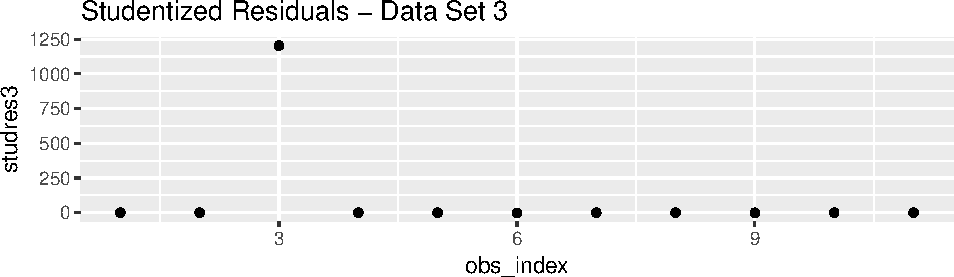
\includegraphics{20190417_residual_diagnostics_files/figure-latex/unnamed-chunk-6-1.pdf}

\begin{Shaded}
\begin{Highlighting}[]
\CommentTok{# confirm observation 3 is the one with a big Y!}
\NormalTok{anscombe}\OperatorTok{$}\NormalTok{y3[}\DecValTok{3}\NormalTok{]}
\end{Highlighting}
\end{Shaded}

\begin{verbatim}
## [1] 12.74
\end{verbatim}

\begin{verbatim}
## Warning: Removed 1 rows containing missing values (geom_point).
\end{verbatim}

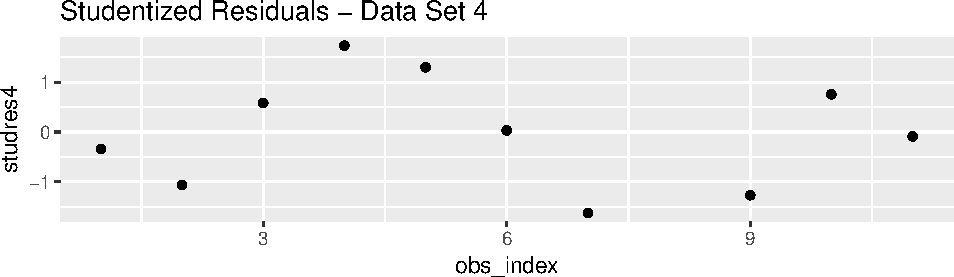
\includegraphics{20190417_residual_diagnostics_files/figure-latex/unnamed-chunk-8-1.pdf}

Looks OK\ldots{} what's up with that warning?

\begin{Shaded}
\begin{Highlighting}[]
\NormalTok{anscombe}\OperatorTok{$}\NormalTok{studres4}
\end{Highlighting}
\end{Shaded}

\begin{verbatim}
##           1           2           3           4           5           6 
## -0.34104165 -1.06669299  0.58216636  1.73514504  1.30031318  0.03136768 
##           7           8           9          10          11 
## -1.62381807         NaN -1.27046922  0.75677904 -0.08931624
\end{verbatim}

\begin{Shaded}
\begin{Highlighting}[]
\NormalTok{anscombe}\OperatorTok{$}\NormalTok{h4}
\end{Highlighting}
\end{Shaded}

\begin{verbatim}
##   1   2   3   4   5   6   7   8   9  10  11 
## 0.1 0.1 0.1 0.1 0.1 0.1 0.1 1.0 0.1 0.1 0.1
\end{verbatim}

\newpage

\subsection{Cook's Distance}\label{cooks-distance}

\begin{itemize}
\tightlist
\item
  Measures how different predicted values for all observations are when
  observation \(i\) is or is not used for model estimation
\item
  Fit model using all observations; get predicted values \(\hat{Y}_j\)
  for each \(j = 1, \ldots, n\)
\item
  Fit model using all observations \textbf{other than} \(i\); get
  predicted values \(\hat{Y}_{j(i)}\) for each \(j = 1, \ldots, n\)
\item
  \(D_i = \frac{\sum_{j = 1}^n (\hat{Y}_{j(i)} - \hat{Y}_j)^2}{p \hat{\sigma}^2}\)
\item
  As a very rough guide, \(D_i > 1\) indicates an observation is worth
  looking into more
\end{itemize}

Plots of Cook's distance vs.~observation index (code will be shown
later)

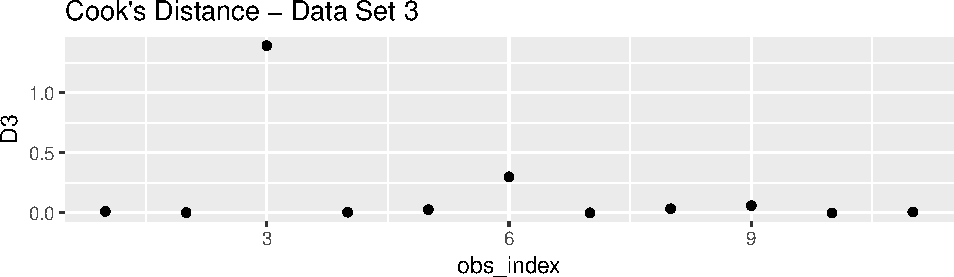
\includegraphics{20190417_residual_diagnostics_files/figure-latex/unnamed-chunk-10-1.pdf}

\begin{Shaded}
\begin{Highlighting}[]
\CommentTok{# confirm observation 3 is the one with a big Y!}
\NormalTok{anscombe}\OperatorTok{$}\NormalTok{y3[}\DecValTok{3}\NormalTok{]}
\end{Highlighting}
\end{Shaded}

\begin{verbatim}
## [1] 12.74
\end{verbatim}

\begin{verbatim}
## Warning: Removed 1 rows containing missing values (geom_point).
\end{verbatim}

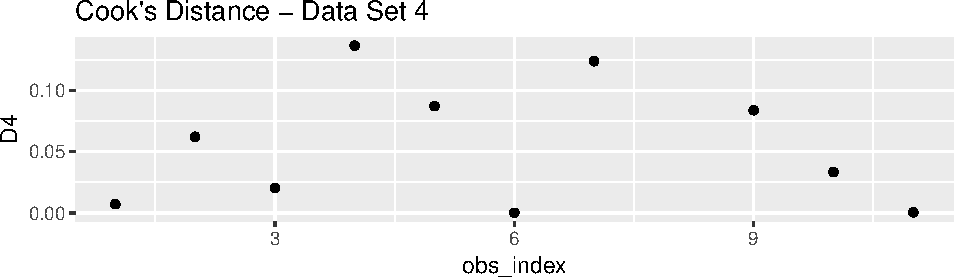
\includegraphics{20190417_residual_diagnostics_files/figure-latex/unnamed-chunk-12-1.pdf}

Looks OK\ldots{} what's up with that warning?

\begin{Shaded}
\begin{Highlighting}[]
\NormalTok{anscombe}\OperatorTok{$}\NormalTok{D4}
\end{Highlighting}
\end{Shaded}

\begin{verbatim}
##            1            2            3            4            5 
## 7.165166e-03 6.225950e-02 2.032144e-02 1.367179e-01 8.723799e-02 
##            6            7            8            9           10 
## 6.148813e-05 1.239465e-01          NaN 8.394407e-02 3.340334e-02 
##           11 
## 4.980902e-04
\end{verbatim}

\begin{Shaded}
\begin{Highlighting}[]
\NormalTok{anscombe}\OperatorTok{$}\NormalTok{h4}
\end{Highlighting}
\end{Shaded}

\begin{verbatim}
##   1   2   3   4   5   6   7   8   9  10  11 
## 0.1 0.1 0.1 0.1 0.1 0.1 0.1 1.0 0.1 0.1 0.1
\end{verbatim}

\newpage

\subsection{R Code: Manual Plots}\label{r-code-manual-plots}

\begin{itemize}
\tightlist
\item
  Every statistical software package will give you different plots by
  default
\item
  Our book suggests the plots we've looked at so far, which are not the
  defaults for R/require more code to create:
\end{itemize}

\begin{Shaded}
\begin{Highlighting}[]
\NormalTok{anscombe <-}\StringTok{ }\NormalTok{anscombe }\OperatorTok
\StringTok{  }\KeywordTok{mutate}\NormalTok{(}
    \DataTypeTok{obs_index =} \KeywordTok{row_number}\NormalTok{(),}
    \DataTypeTok{h3 =} \KeywordTok{hatvalues}\NormalTok{(fit3),}
    \DataTypeTok{studres3 =} \KeywordTok{rstudent}\NormalTok{(fit3),}
    \DataTypeTok{D3 =} \KeywordTok{cooks.distance}\NormalTok{(fit3)}
\NormalTok{  )}

\KeywordTok{ggplot}\NormalTok{(}\DataTypeTok{data =}\NormalTok{ anscombe, }\DataTypeTok{mapping =} \KeywordTok{aes}\NormalTok{(}\DataTypeTok{x =}\NormalTok{ obs_index, }\DataTypeTok{y =}\NormalTok{ h3)) }\OperatorTok{+}
\StringTok{  }\KeywordTok{geom_point}\NormalTok{() }\OperatorTok{+}
\StringTok{  }\KeywordTok{geom_hline}\NormalTok{(}\DataTypeTok{yintercept =} \DecValTok{2} \OperatorTok{*}\StringTok{ }\DecValTok{2} \OperatorTok{/}\StringTok{ }\KeywordTok{nrow}\NormalTok{(anscombe)) }\OperatorTok{+}
\StringTok{  }\KeywordTok{ylim}\NormalTok{(}\DecValTok{0}\NormalTok{, }\DecValTok{1}\NormalTok{) }\OperatorTok{+}
\StringTok{  }\KeywordTok{ggtitle}\NormalTok{(}\StringTok{"Leverage - Data Set 3"}\NormalTok{)}
\end{Highlighting}
\end{Shaded}

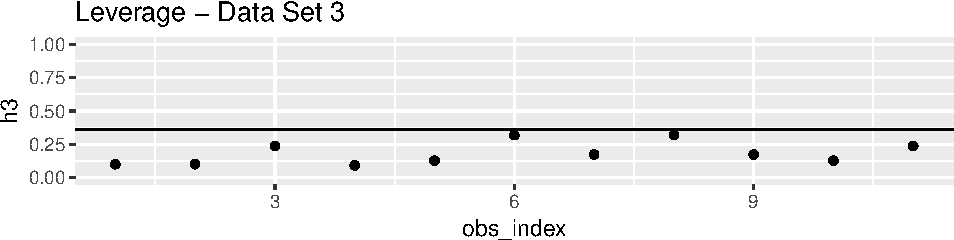
\includegraphics{20190417_residual_diagnostics_files/figure-latex/unnamed-chunk-14-1.pdf}

\begin{Shaded}
\begin{Highlighting}[]
\KeywordTok{ggplot}\NormalTok{(}\DataTypeTok{data =}\NormalTok{ anscombe, }\DataTypeTok{mapping =} \KeywordTok{aes}\NormalTok{(}\DataTypeTok{x =}\NormalTok{ obs_index, }\DataTypeTok{y =}\NormalTok{ studres3)) }\OperatorTok{+}
\StringTok{  }\KeywordTok{geom_point}\NormalTok{() }\OperatorTok{+}
\StringTok{  }\KeywordTok{ggtitle}\NormalTok{(}\StringTok{"Studentized Residuals - Data Set 3"}\NormalTok{)}
\end{Highlighting}
\end{Shaded}

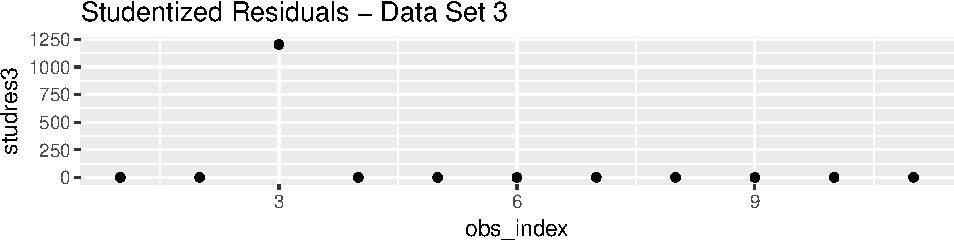
\includegraphics{20190417_residual_diagnostics_files/figure-latex/unnamed-chunk-14-2.pdf}

\begin{Shaded}
\begin{Highlighting}[]
\KeywordTok{ggplot}\NormalTok{(}\DataTypeTok{data =}\NormalTok{ anscombe, }\DataTypeTok{mapping =} \KeywordTok{aes}\NormalTok{(}\DataTypeTok{x =}\NormalTok{ obs_index, }\DataTypeTok{y =}\NormalTok{ D3)) }\OperatorTok{+}
\StringTok{  }\KeywordTok{geom_point}\NormalTok{() }\OperatorTok{+}
\StringTok{  }\KeywordTok{ggtitle}\NormalTok{(}\StringTok{"Cook's Distance - Data Set 3"}\NormalTok{)}
\end{Highlighting}
\end{Shaded}

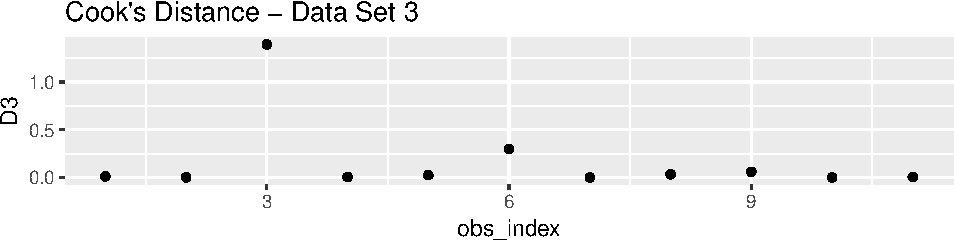
\includegraphics{20190417_residual_diagnostics_files/figure-latex/unnamed-chunk-14-3.pdf}

\newpage

\subsection{R Code: Default Plots}\label{r-code-default-plots}

You can get a set of different diagnostic plots more easily, but I find
the plot involving Cook's distance and Leverage less intuitive:

\begin{Shaded}
\begin{Highlighting}[]
\KeywordTok{plot}\NormalTok{(fit3)}
\end{Highlighting}
\end{Shaded}

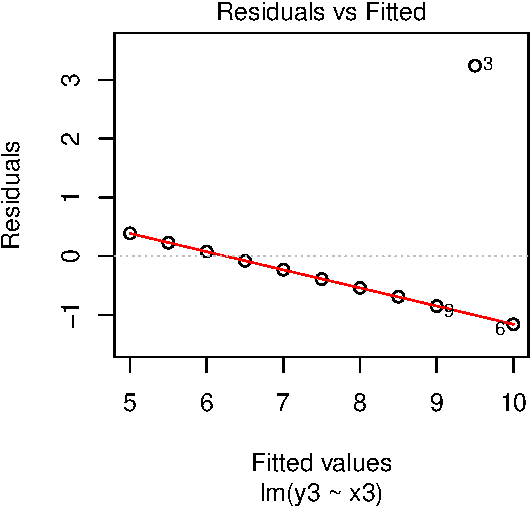
\includegraphics{20190417_residual_diagnostics_files/figure-latex/unnamed-chunk-15-1.pdf}
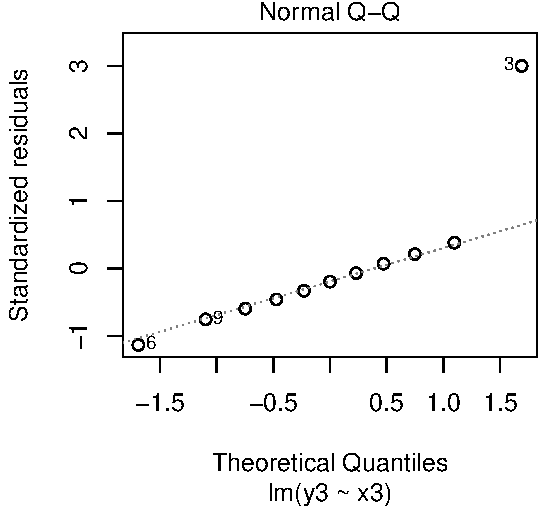
\includegraphics{20190417_residual_diagnostics_files/figure-latex/unnamed-chunk-15-2.pdf}
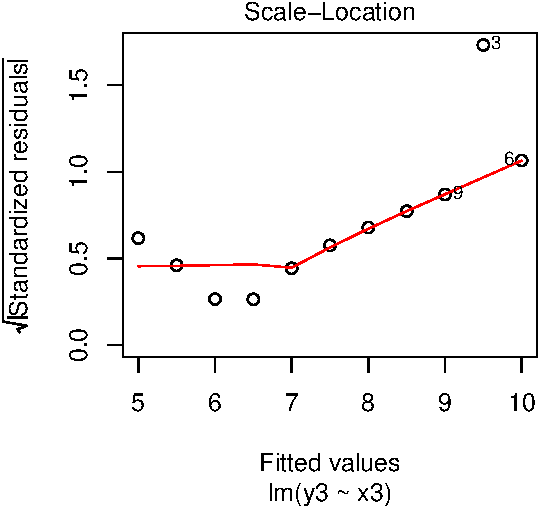
\includegraphics{20190417_residual_diagnostics_files/figure-latex/unnamed-chunk-15-3.pdf}
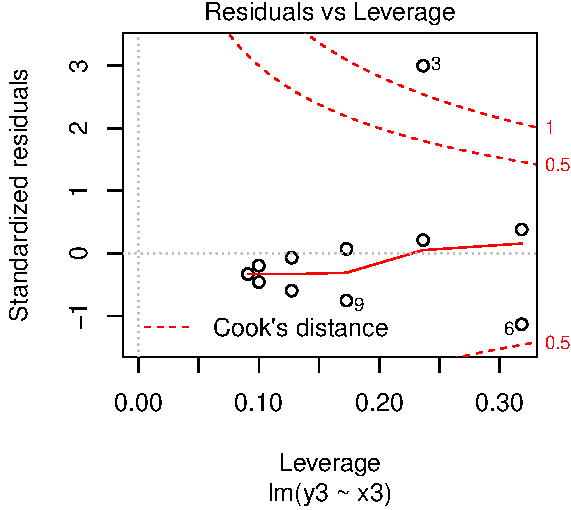
\includegraphics{20190417_residual_diagnostics_files/figure-latex/unnamed-chunk-15-4.pdf}

Note: to get the plots to all show up in the knitted pdf, I had to set
figure height and width in the code chunk declaration:

\begin{Shaded}
\begin{Highlighting}[]
\NormalTok{```\{r, fig.height = 4, fig.width = 4\}}
\end{Highlighting}
\end{Shaded}


\end{document}
